%% LaTeX-Beamer template for KIT design
%% by Erik Burger, Christian Hammer
%% title picture by Klaus Krogmann
%%
%% version 2.1
%%
%% mostly compatible to KIT corporate design v2.0
%% http://intranet.kit.edu/gestaltungsrichtlinien.php
%%
%% Problems, bugs and comments to
%% burger@kit.edu

\documentclass[18pt]{beamer}
\usepackage[utf8x]{inputenc}
\usepackage{units}
\usepackage{booktabs}

%% CUSTOM
\usepackage{amsmath}
\usepackage{algpseudocode}

%% Definitions
\DeclareMathOperator{\div2}{div}
\renewcommand{\algorithmicrequire}{\textbf{Input:}}
\renewcommand{\algorithmicensure}{\textbf{Output:}}
\algnewcommand\algorithmicto{\textbf{to}}
\algrenewtext{For}[3]{\algorithmicfor\ $#1 \gets #2$ \algorithmicto\ $#3$ \algorithmicdo}
\algnewcommand\algorithmicod{\textbf{od}}
\algrenewtext{EndWhile}{\algorithmicod}
\algrenewtext{EndFor}{\algorithmicod}
%\AtBeginSection[]{%
%\begin{frame}<beamer> % do nothing in handouts
%    \frametitle{Überblick}
%    \tableofcontents[sectionstyle=show/shaded,
%    subsectionstyle=show/show/hide]
%\end{frame}
%}
%\AtBeginSubsection[]{%
%\begin{frame}<beamer> % do nothing in handouts
%    \frametitle{Überblick}
%    \tableofcontents[sectionstyle=show/shaded,
%    subsectionstyle=show/shaded/hide]
%\end{frame}
%}

%% SLIDE FORMAT

% use 'beamerthemekit' for standard 4:3 ratio
% for widescreen slides (16:9), use 'beamerthemekitwide'

\usepackage{templates/beamerthemekit}
%\usepackage{templates/beamerthemekitwide}

 %% TITLE PICTURE

 % if a custom picture is to be used on the title page, copy it into the 'logos'
 % directory, in the line below, replace 'mypicture' with the 
 % filename (without extension) and uncomment the following line
 % (picture proportions: 63 : 20 for standard, 169 : 40 for wide
 % *.eps format if you use latex+dvips+ps2pdf, 
 % *.jpg/*.png/*.pdf if you use pdflatex)


 \titleimage{banner}
 
 
%% Define some colors:
\definecolor{darkblue}{rgb}{0,0,.5}
\definecolor{darkgreen}{rgb}{0,.5,0}

 %% TITLE LOGO

 % for a custom logo on the front page, copy your file into the 'logos'
 % directory, insert the filename in the line below and uncomment it

\titlelogo{logo_150x150}
 
 % (*.eps format if you use latex+dvips+ps2pdf,
 % *.jpg/*.png/*.pdf if you use pdflatex)
 
 %% TikZ INTEGRATION
 
 % use these packages for PCM symbols and UML classes
 % \usepackage{templates/tikzkit}
 % \usepackage{templates/tikzuml}
 
 % the presentation starts here
 
\author{Dominik Muth - dominik.muth@student.kit.edu}
\institute{Institut f\"ur Informatik}


\title[Tutorium 10]{GBI Tutorium Nr. $2^5$}
\subtitle{Tutorium 10}
\date{9. Januar 2013}

% Bibliography



\begin{document}

	%title page
	\begin{frame}
		\titlepage
	\end{frame}

	%table of contents
	\begin{frame}{Outline/Gliederung}
		\tableofcontents
	\end{frame}	
		
	
	
	\section{Wiederholung} 
	\begin{frame} {Wiederholung - Quiz}
		\begin{itemize}
			
			\item Bei einem Mealy Automat hängt die Ausgabe nur vom Zustand ab.
			\only<2-> {\color{red}$X$}\\
			\color{black}
			\item Seien $L_1$ und $L_2$ formale Sprachen. $L_1^* = L_2^* \Rightarrow L_1 = L_2$
			\only<3-> {\color{red}$X$}\\
			\color{black}
			
			\item Jeder Moore Automat lässt sich in einen Mealy Automat unwandeln. 
			\only<4-> {\color{darkgreen}$\surd$}\\
			\color{black}
	
			\item $T(n) = 2T(\frac{n}{2}) + 10n \Rightarrow T(n) \in \Theta(n\, log(n))$
			\only<5-> {\color{darkgreen}$\surd$}\\
			\color{black}
		\end{itemize}
	\end{frame}
	
	
	\begin{frame}{Wiederholung - Formale Sprachen}
		\begin{itemize}
			\item Was war eine formale Sprache?
			\item Geben Sie die formale Sprache für alle ganzen Zahlen an.
		\end{itemize}
	\end{frame}
	
	
	
	\section{Reguläre Ausdrücke}
	
	\begin{frame}{Reguläre Ausdrücke}
		\begin{block}{Was ist das?}
			\pause
			Beschreibt Sprachen.\\
			Die Schreibweise ist ähnlich wie bei formale Sprachen.\\
			Wenn R ein regulärer Ausdruck ist, ist $\langle R\rangle$ die von R produzierte Sprache.
		\end{block}
			\pause
		
		\begin{block}{Wie funktioniert's?}
			\begin{itemize}
			\pause
				\item $|$ = oder
			\pause
				\item $*$ = beliebig viele
			\pause
				\item $()$ = Klammerung
			\end{itemize}
		\end{block}
	\end{frame}
	
	\begin{frame}{Reguläre Ausdrücke}
		
		\begin{exampleblock}{Beispiel}
			Sei $R = (ab|b)*$ dann enthält $\langle R\rangle$ alle Wörter aus $\{a,b\}$ bei denen nach einem a immer ein b kommt: $(\{ab\}\bigcup \{b\})^*$\\
			\vspace{10pt}
			\pause
			$(a|b)*abb(a|b)*$: . . . $\langle R\rangle$ entält genau die Wörter, in denen das Teilwort abb vorkommt.\\
			\vspace{10pt}
			\pause
			$a*\!* = a*$\\
			\vspace{10pt}
			$\langle \emptyset *\rangle =\langle \emptyset \rangle ^* = \{\}^* = \{\epsilon\} $
		\end{exampleblock}
	\end{frame}
	
	
	\begin{frame}{Reguläre Ausdrücke - Aufgaben}
		\begin{itemize}
			\item Geben sie einen regulären Ausdruck $R_1$ an, für welchen gilt: $\langle R_1\rangle$ enthält alle Wörter bei denen kein a vor einem b kommt.
			\item Geben sie einen endlichen Akzeptor an, welcher Wörter aus $\langle R_1\rangle$ akzeptiert.
			\item Welche Wörter akzeptiert folgender regulärer Ausdruck:\\
				$R = R_2(aaR_2bb|bbR_2aa)R_2$ mit $R_2 = aa|bb|ab|ba$?
		\end{itemize}
	\end{frame}
	
	
	\begin{frame}{Reguläre Ausdrücke - Aufgaben}
		\begin{center}
			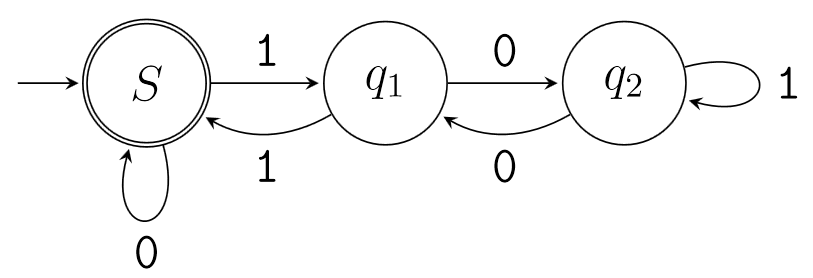
\includegraphics[scale=.3]{graphics/11/akzeptor1.png}
		\end{center}
		\begin{enumerate}
			\item Welche Wörter Akzeptiert der Akzeptor?\\
				\visible<2-> {\color{darkgreen}Durch 3 teilbare Binärzahlen und $\epsilon$\color{black}}
			\item Geben Sie R an, damit gilt: $L(A)= \langle R \rangle$\\
				\visible<3-> {\color{darkgreen}$(0|1(01∗0)∗1)∗$\color{black}}
		\end{enumerate}
	\end{frame}
	
	
	\section{Rechtslineare Grammatiken} 
	\begin{frame}{Rechtslineare Grammatiken}
		\begin{itemize}
			\item Wie waren kontextfreie Grammatiken definiert?
			\item Was sind lineare Grammatiken?
			\item Wie sieht eine rechtslineare Grammatik aus?
		\end{itemize}
	\end{frame}
	
	
	\begin{frame}{Rechtslineare Grammatiken} 
		\begin{block}{Erläuterung}
			Rechtslineare Grammatiken sind genauso definiert wie kontextfreie Grammatiken:\\
			$G=(N,T,S,P)$\\
			allerdings gilt bei rechtslinearen Grammatiken für P:\\
			$\forall w_1 \rightarrow w_2 \in P : w_1 \in N \land w_2 \in \{\epsilon\} \bigcup T^* \bigcup T^*N$
		\end{block}
	\end{frame}
	
	
	\begin{frame}{Rechtslineare Grammatiken} 
		\begin{exampleblock}{Beispiel}
			Die Rechtslineare Grammatik welche Wörter ohne bb produziert:\\
			\vspace{10pt}
			$G = (\{S, B\},\{a,b\}, S, P)$\\
			$P = \{ S \rightarrow aS | bB | \epsilon,$\\
			\hspace{27pt}$B \rightarrow aS | \epsilon \}$
		\end{exampleblock}
		
		\visible<2-> {Kann man diese Grammatik noch vereinfachen?}
	\end{frame}
	
	
	\begin{frame}{Rechtslineare Grammatiken - Aufgaben} 
		Geben sie folgende rechtslineare Grammatiken an:
		\begin{itemize}
			\item $L(G_1) = \{w\in \{a,b\}^∗|N_a(w) mod 2 = 1\}$
			\item $L(G_2) = (\langle 0|1(01∗0)∗1)∗\rangle$
			\item $L(G_3) = \{w \in \{a,b\}^*|$w enthält weder das Teilwort aa noch das Teilwort bb$\}$
		\end{itemize}
	\end{frame}
	
	
	\section{Klausuraufgabe}	
	
	\begin{frame}{Klausuraufgabe}
		Geben Sie zu folgenden regulären Ausdrücken $R_i, i\in \{1,2\} $jeweils einen endlichen Akzeptor $A_i$ (wie in der Vorlesung definiert) an, so dass $L(A) = \langle R \rangle$.\\
		\begin{itemize}
			\item $R_1 = (aa)*b(aaa)*$
			\item $R_2 = (a|ba)*(b|ab)(b|ab)*$
		\end{itemize}
	\end{frame}
	
	
	\section{Fragen}
	\begin{frame} {Fragen}
		\begin{itemize}
			\item Fragen zum Stoff?
			\item Fragen zum n\"achsten \"Ubungsblatt?
			\item Generelle Fragen?
			\item Feedback?
		\end{itemize}
	\end{frame}	
		
		
	\begin{frame} {EOF}
		\begin{center}
			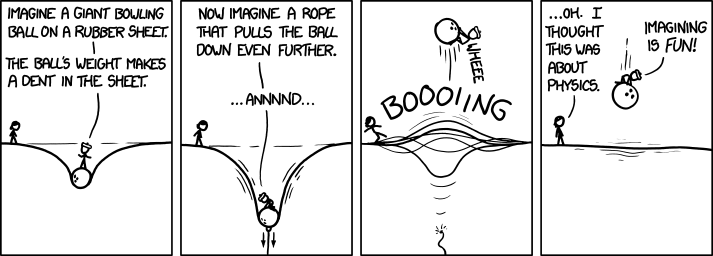
\includegraphics[scale=0.45]{graphics/eof11.png}\\
			\tiny $source: http://imgs.xkcd.com/comics/rubber\_sheet.png$
		\end{center}
	\end{frame}

\end{document}
